% !TEX TS-program = xelatex
% !TEX encoding = UTF-8 Unicode
% !Mode:: "TeX:UTF-8"

\documentclass{resume}
\usepackage{graphicx}
\usepackage{tabu}
\usepackage{tabularx, booktabs}
\usepackage{multirow}
\usepackage{makecell}
\usepackage{zh_CN-Adobefonts_external} % Simplified Chinese Support using external fonts (./fonts/zh_CN-Adobe/)
% \usepackage{NotoSansSC_external}
% \usepackage{NotoSerifCJKsc_external}
% \usepackage{zh_CN-Adobefonts_internal} % Simplified Chinese Support using system fonts
\usepackage{linespacing_fix} % disable extra space before next section
\usepackage{cite}

\begin{document}
\pagenumbering{gobble} % suppress displaying page number

\renewcommand\arraystretch{1.5}
\begin{tabular}{p{13cm} p{4cm}}
  \textbf{\huge 方缙} & \multirowcell{5}{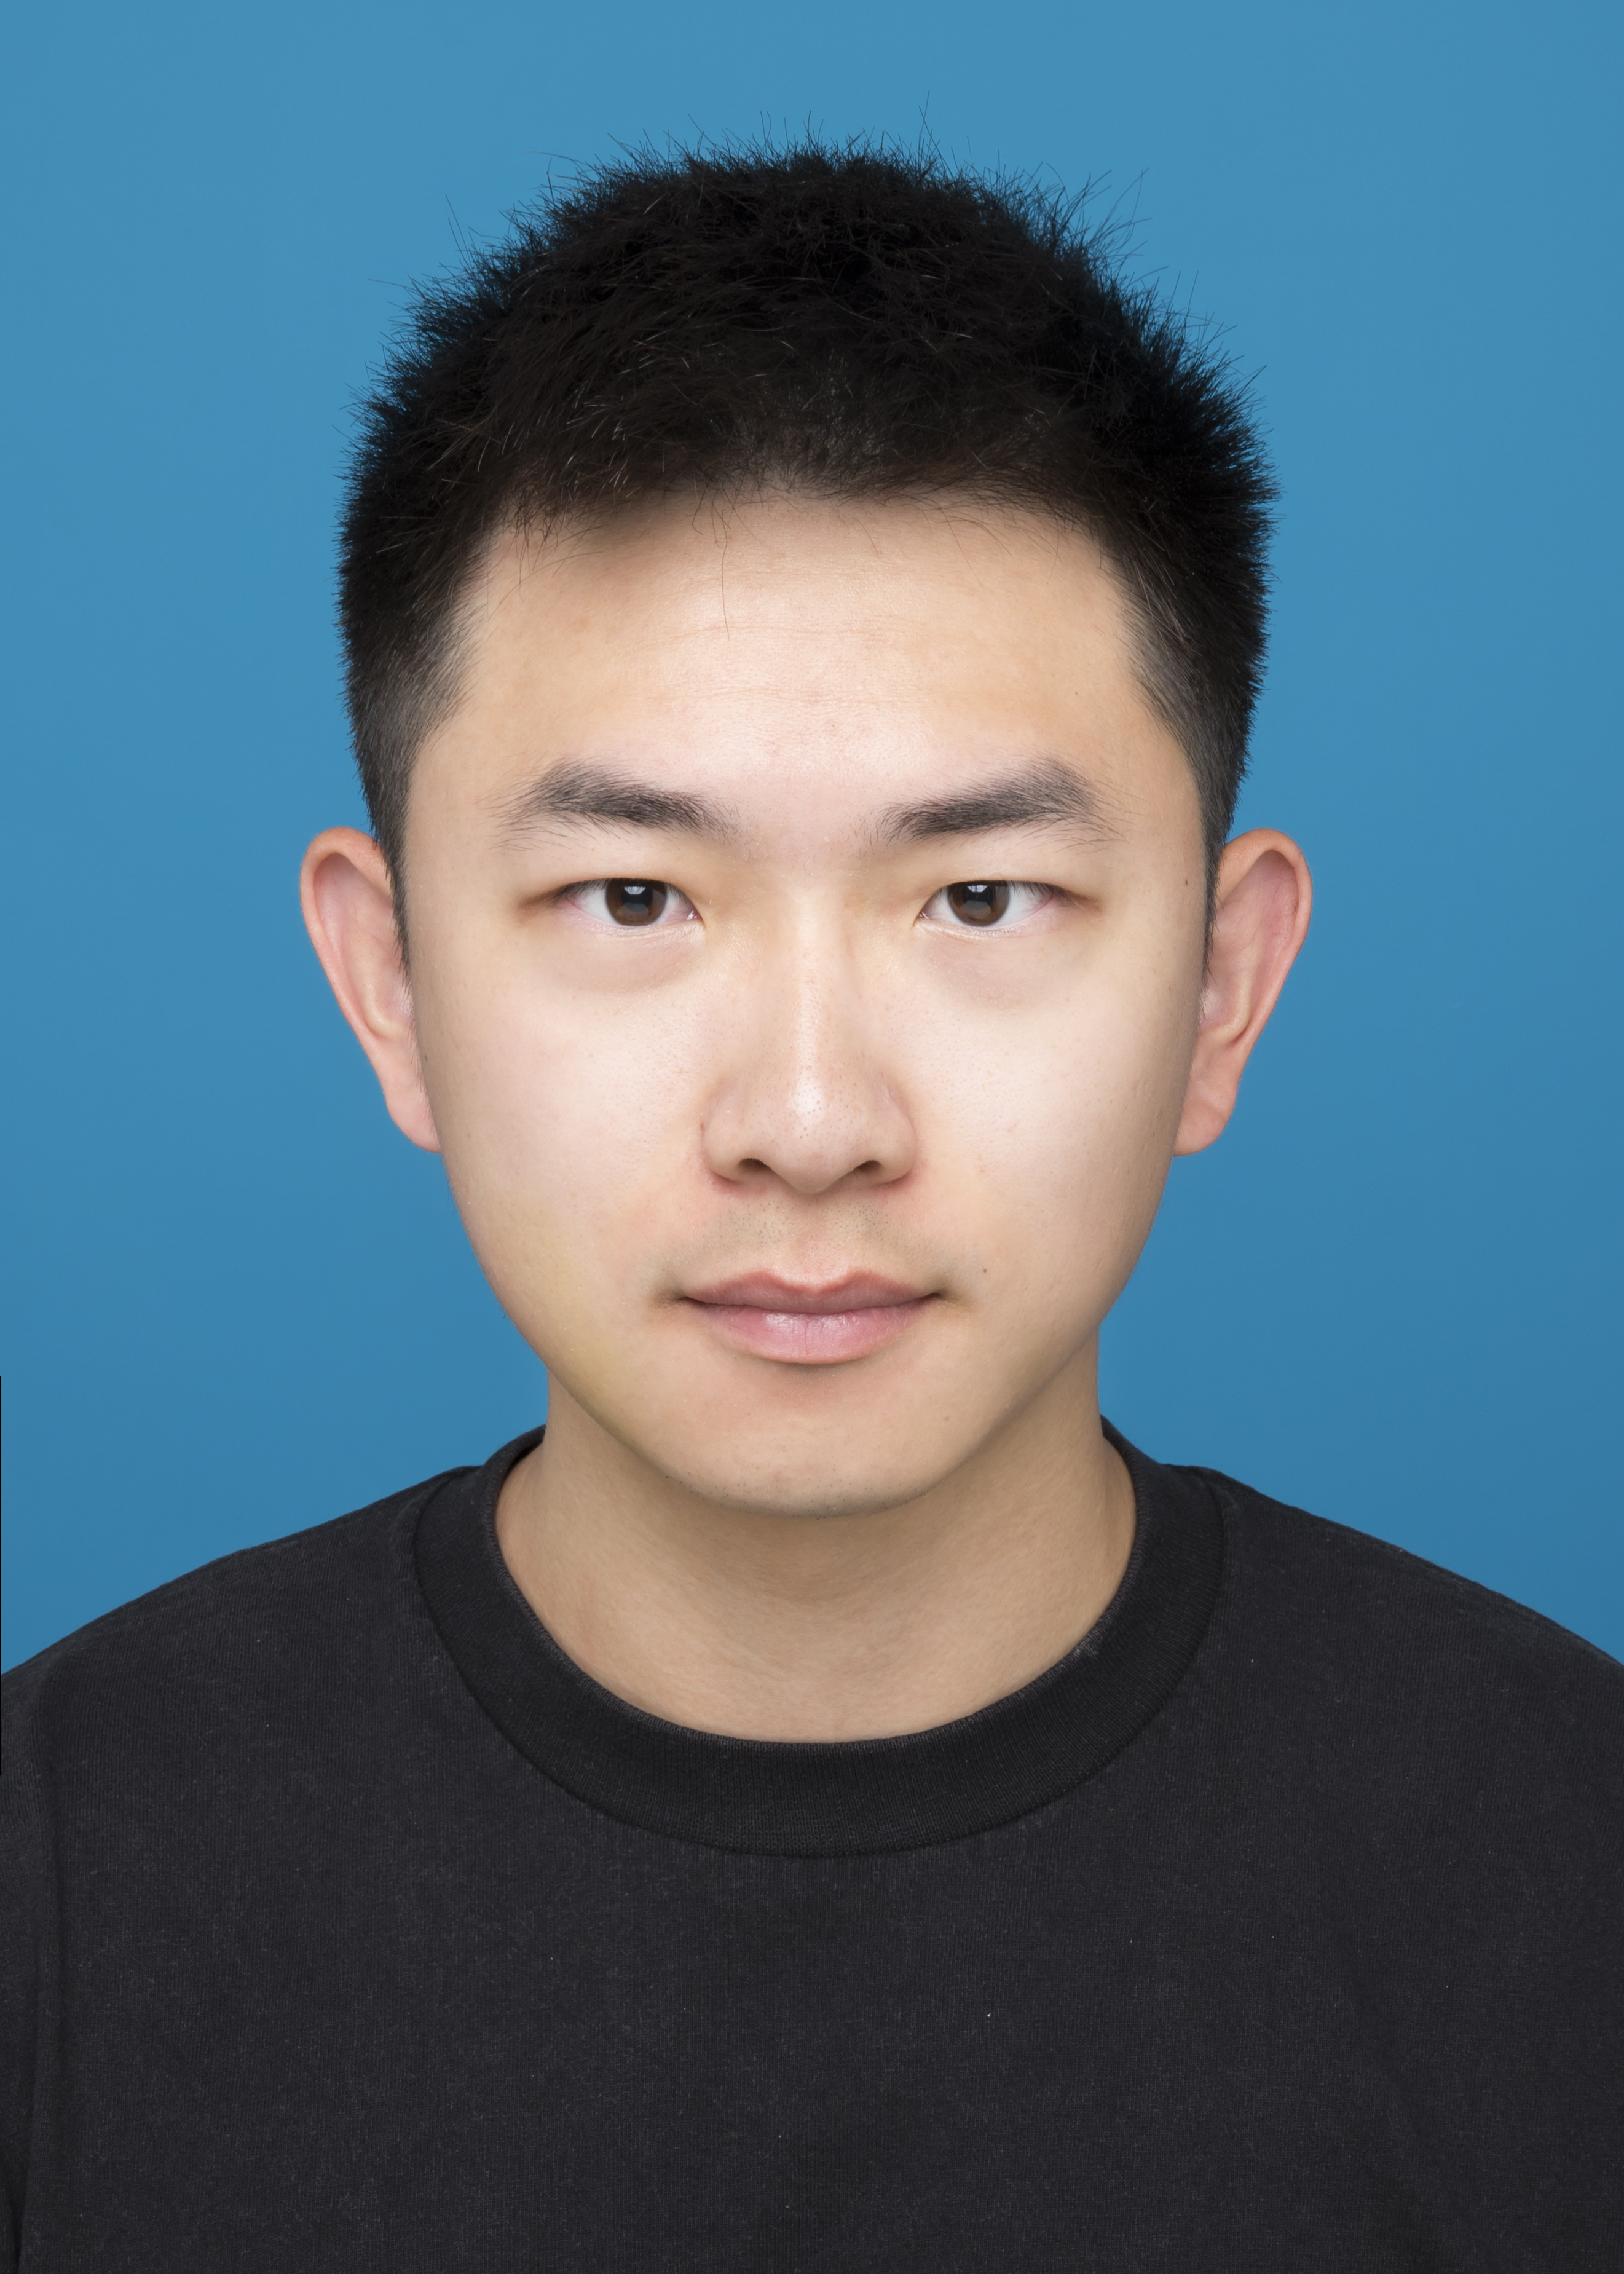
\includegraphics[scale=0.1]{avatar}}\\
  \email{fangjin98@mail.ustc.edu.cn} & \\
  \phone{(+86) 181-5566-1676} & \\
  \homepage[www.fangjin.site]{www.fangjin.site} & \\
\end{tabular}


% \name{方缙}

% \basicInfo{
%   \email{fangjin98@mail.ustc.edu.cn} \textperiodcentered\ 
%   \phone{(+86) 181-5566-1676} \textperiodcentered\ 
%   \homepage[www.fangjin.site]{www.fangjin.site}
% }

\section{教育背景}

\datedsubsection{\textbf{中国科学技术大学} \qquad \textit{硕博连读} \qquad 计算机科学与技术}{2020.9-2025.6 (预计)}
\begin{itemize}
  \item 研究方向: 数据中心网络、可编程网络、分布式训练、在网计算
  \item 导师:徐宏力、赵功名
\end{itemize}

\datedsubsection{\textbf{湖南大学} \qquad \qquad \qquad \textit{学士} \qquad \qquad 计算机科学与技术}{2016.9-2020.6}
\begin{itemize}
  \item 湖南大学优秀毕业论文
\end{itemize}

\section{项目经历}

\datedsubsection{\textbf{优化光网络下分布式训练节点部署工作}}{华为2012中央研究院,合肥}
\datedsubsection{\textit{技术点负责人}}{2023.12-至今}
\begin{itemize}[parsep=0.5ex]
  \item 大模型的分布式训练任务具有算力亲和性,然而算力由多层机间网络互联、带宽异构,导致跨节点网络成为训练瓶颈
  \item 调研现有大模型任务部署和算力调度优化方案,熟悉常见模型并行和数据并行方法
  \item 调研现有模型压缩工作,熟悉稀疏模型训练优化方法
  \item 对不同集合通信算法下的物理节点和逻辑节点通信模式建模,分析通信拓扑、链路对任务训练时间的影响
  \item 设计任务部署算法降低光网络下跨机架任务通信量
\end{itemize}

\datedsubsection{\textbf{下一代云原生 SDN 平台开发测试}}{华为美研院 (Futurewei),远程}
\datedsubsection{\textit{项目开发}}{2021.6-2021.9}
\begin{itemize}[parsep=0.5ex]
  \item 针对大规模测试实验编写自动化测试bash脚本
  \item 基于 C++ 编写端到端虚拟网络控制面测试案例
  \item 基于 C++ 开发 Pulsar 消息队列订阅特性 (\href{https://github.com/futurewei-cloud/alcor-control-agent/pull/274}{\textit{PR \#274}})
\end{itemize}

\section{科研经历}

\datedsubsection{\textbf{基于可编程网络实现精准模拟网络故障}}{中科大苏高院,苏州}
\datedsubsection{\textit{主要开发者}}{2022.12-2023.9}
\begin{itemize}[parsep=0.5ex]
  \item 基于端主机的故障注入难以覆盖大量复杂网络故障场景,且无法针对应用流量精准注入故障
  \item 基于可编程控制面设计并实现用户友好的多后端故障注入系统,提供一系列参数供用户自定义流量协议
  \item 针对流依赖和流过滤,设计一个解析器生成算法,能够根据用户指示生成对应数据面程序
  \item 针对多租户和路由路径,形式化故障注入点选择问题
  \item 针对异构多后端网络设备,基于 P4 TNA 和 PSA 架构实现多种网络功能,系统资源消耗小于10\%
  \item 在4个流行的分布式系统任务 (Horovod, Redis, RDMA, Kafka) 中测试该系统并验证故障注入效果
\end{itemize}

\datedsubsection{\textbf{使用可编程交换机加速分布式模型训练}}{之江实验室,杭州}
\datedsubsection{\textit{主要开发者}}{2022.6-2022.9}
\begin{itemize}[parsep=0.5ex]
  \item 大规模分布式模型训练具有通信瓶颈,该项目通过可编程交换机在网内聚合梯度以降低通信量,从而加速分布式模型训练
  \item 针对流量可变性,设计基于随机舍入算法解决网内聚合场景下的梯度路由问题
  \item 基于 Pytorch 实现包含 8 台服务器的 PS 架构分布式模型训练原型系统,主机间通过自定义协议进行通信 (\href{https://github.com/Fangjin98/distributed-training-INA/}{\textit{链接}})
  \item 基于 Intel Tofino 可编程交换机实现网内聚合逻辑,并与主机端实现协同训练
  \item 相比较现有方案,降低分布式训练通信负载 $81.2\%$
\end{itemize}

\datedsubsection{\textbf{面向边缘云考虑鲁棒性的虚拟网络功能部署算法}}{中科大,合肥}
\datedsubsection{\textit{主要开发者}}{2021.2-2021.6}
\begin{itemize}[parsep=0.5ex]
  \item 边缘云的性能往往受到恶意用户和虚拟网络功能 (VNF)的影响,本文考虑限制恶意用户和 VNF 影响范围,提升边缘云鲁棒性
  \item 考虑到VNF部署和用户请求调度往往在不同时间维度,设计了一个离线算法决策VNF部署以及在线算法执行请求调度
  \item 基于 Python 实现了包含 6 台 Nvidia Jetson Tx2s 和 20 台 Raspberry Pis 的原型系统 (\href{https://github.com/Fangjin98/reveal-src}{\textit{链接}})
  \item 实验结果表明,在异常情况下该方案能够提升网络吞吐率 $57\%$
\end{itemize}

\datedsubsection{\textbf{基于 FPGA 高层次综合实现 LSTM 模型}}{湖南大学,长沙}
\datedsubsection{\textit{本科毕设项目}}{2019.6-2020.1}
\begin{itemize}[parsep=0.5ex]
  \item 基于 Keras 训练 LSTM 模型以预测核电站反应堆蒸汽压力系统
  \item 基于 C++ 移植训练好的 LSTM 模型至 Pynq-Z2 开发版 (\href{https://github.com/Fangjin98/vivado-hls-rnn}{\textit{链接}})
  \item 相比较软件方案,能够减少模型推理时间 90 倍
  \item \textit{获得湖南大学优秀毕业论文奖}
\end{itemize}

\section{学术成果}

\begin{enumerate}[parsep=0.5ex]
  \item \textbf{J. Fang}, G. Zhao, H. Xu, Z. Yu, B. Shen, X. Li, \textit{Accelerating Distributed Training with Collaborative In-network Aggregation}, IEEE/ACM Transactions on Networking (\textbf{ToN}), 2024, CCF A
  \item \textbf{J. Fang}, G. Zhao, H. Xu, C. Wu, Z. Yu, \textit{GRID: Gradient Routing with In-network Aggregation for Distributed Training}, IEEE/ACM Transactions on Networking (\textbf{ToN}), 2023, CCF A
  \item \textbf{J. Fang}, G. Zhao, H. Xu, Z. Yu, B. Shen, X. Li, \textit{GOAT: Gradient Scheduling with Collaborative In-Network Aggregation for Distributed Training}, IEEE/ACM International Symposium on Quality of Service (\textbf{IWQoS}), 2023, CCF B
  \item \textbf{J. Fang}, G. Zhao, H. Xu, H. Tu, H. Wang, \textit{Reveal: Robustness-Aware VNF Placement and Request Scheduling in Edge Clouds}, Computer Networks (\textbf{ComNet}), 2023, CCF B
  \item (在投) \textbf{J. Fang}, G. Zhao, H. Xu, Z. Yu, J. Jiang, F. Zeng, \textit{Injecting Failure for Success: Towards General, Flexible and Efficient Network Fault Injection}, USENIX ATC, 2024, CCF A
  \item J. Liu, Y. Zhai, G. Zhao, H. Xu, \textbf{J. Fang}, Z. Zeng, Y. Zhu, InArt: In-Network Aggregation with Route Selection for Accelerating Distributed Training, International World Wide Web Conference (\textbf{WWW}), 2024, CCF A
  \item 赵功名, \textbf{方缙}, 徐宏力, 吴昌博, \textit{PS架构下基于可编程交换机的梯度调度方法和装置}, 已授权
  \item 徐宏力, \textbf{方缙}, 赵功名, 凃化清, 汪海波, \textit{一种边缘云系统中的VNF部署调度方法}, 已公开
\end{enumerate}

\section{奖项荣誉}

\begin{itemize}[parsep=0.5ex]
  \item \datedline{中国电科十四所国睿奖学金}{2023}
  \item \datedline{英特尔 P4 中国黑客松优胜奖}{2022}
  \item \datedline{一等学业奖学金(博士)$\times 2$}{2022, 2023}
  \item \datedline{一等学业奖学金(硕士)$\times 2$}{2020, 2021}
\end{itemize}

\section{专业技能}

\begin{itemize}[parsep=0.5ex]
  \item 编程语言: Python, C/C++, P4, C\#, Swift
  \item 开发框架: Pytorch, p4c, eBPF, Mininet
\end{itemize}

\end{document}
